\let\negmedspace\undefined
\let\negthickspace\undefined
\documentclass[journal]{IEEEtran}
\usepackage[a5paper, margin=10mm, onecolumn]{geometry}
%\usepackage{lmodern} % Ensure lmodern is loaded for pdflatex
\usepackage{tfrupee} % Include tfrupee package

\setlength{\headheight}{1cm} % Set the height of the header box
\setlength{\headsep}{0mm}     % Set the distance between the header box and the top of the text

\usepackage{gvv-book}
\usepackage{gvv}
\usepackage{cite}
\usepackage{amsmath,amssymb,amsfonts,amsthm}
\usepackage{algorithmic}
\usepackage{graphicx}
\usepackage{textcomp}
\usepackage{xcolor}
\usepackage{txfonts}
\usepackage{listings}
\usepackage{enumitem}
\usepackage{mathtools}
\usepackage{gensymb}
\usepackage{comment}
\usepackage[breaklinks=true]{hyperref}
\usepackage{tkz-euclide}
\usepackage{listings}                                     
\def\inputGnumericTable{}                                 
\usepackage[utf8]{inputenc}                                
\usepackage{color}                                            
\usepackage{array}                                            
\usepackage{longtable}                                       
\usepackage{calc}                                             
\usepackage{multirow}                                         
\usepackage{hhline}                                           
\usepackage{ifthen}                                           
\usepackage{lscape}
\renewcommand{\thefigure}{\theenumi}
\renewcommand{\thetable}{\theenumi}
\setlength{\intextsep}{10pt} % Space between text and floats

\numberwithin{equation}{enumi}
\numberwithin{figure}{enumi}
\renewcommand{\thetable}{\theenumi}

% Marks the beginning of the document
\begin{document}
\bibliographystyle{IEEEtran}

\title{Scientific Calculator Assignment}
\author{EE24BTECH11048-NITHIN.K} 
%\maketitle
%\newpage
%\bigskip
{\let\newpage\relax\maketitle}
\section*{Introduction}
This report details the design and implementation of a scientific calculator based on an Arduino microcontroller. The calculator uses a \textbf{4x4 button matrix} for input, along with \textbf{Shift and Alpha keys} to extend its functionality. The project integrates essential mathematical operations and scientific functions to provide a compact yet powerful computing tool.

\section*{Hardware Components}
\begin{itemize}
\item \textbf{Arduino Uno (ATmega328P)} -- Core processing unit.
\item \textbf{16x2 LCD Display} -- Output device for displaying expressions and results.
\item \textbf{4x4 Button Matrix} -- Input mechanism for digits, operators, and functions.
\item \textbf{Potentiometer} -- Adjusts LCD contrast.
\item \textbf{Power Source} -- 5V supply from USB or battery.
\end{itemize}

\section*{Keypad Layout and Functions}
The calculator features a \textbf{4x4 button layout} with three distinct modes:

\subsection{Normal Mode}
The default mode provides basic arithmetic operations and digit input.

\begin{table}[H]
\centering
\begin{tabular}{|c|c|c|c|c|c|}
\hline
Row & Column 1 & Column 2 & Column 3 & Column 4 & Column 5 \\
\hline
1 & 7 & 8 & 9 & + & D (Delete) \\
2 & 4 & 5 & 6 & - & S (Shift) \\
3 & 1 & 2 & 3 & * & A (Alpha) \\
4 & 0 & . & = & / & C (Clear) \\
\hline
\end{tabular}
\caption{Normal Mode Keypad Layout}
\end{table}

\subsection{Alpha Mode}
Activating the \textbf{Alpha} key changes the button functions to advanced scientific operations.

\begin{table}[H]
\centering
\begin{tabular}{|c|c|c|c|c|c|}
\hline
Row & Column 1 & Column 2 & Column 3 & Column 4 & Column 5 \\
\hline
1 & $\sin{}$ & $\cos{}$ & $\tan{}$ & Power & Backspace \\
2 & $\log{}$ & $\ln{}$ & $e^{x}$ & $\sqrt{}$ & ( \\
3 & $\pi$ & $x^2$ & $x^3$ & 1/x & ) \\
4 & EXP & ANS & M+ & M- & MR \\
\hline
\end{tabular}
\caption{Alpha Mode Keypad Layout}
\end{table}

\subsection{Shift Mode}
Pressing the \textbf{Shift} key modifies the button functionality to perform additional mathematical operations.

\begin{table}[H]
\centering
\begin{tabular}{|c|c|c|c|c|c|}
\hline
Row & Column 1 & Column 2 & Column 3 & Column 4 & Column 5 \\
\hline
1 & asin & acos & atan & $y^{x}$ & CLR \\
2 & $10^{x}$ & e & abs & cbrt (Cube Root) & [ \\
3 & deg & rad & mod & ! & ] \\
4 & HEX & DEC & BIN & OCT & MC \\
\hline
\end{tabular}
\caption{Shift Mode Keypad Layout}
\end{table}

\section*{Software Implementation}
The calculator software is developed in \textbf{C for Arduino}, utilizing efficient algorithms for function calculations. The logic handles button presses, function execution, and result display.

\subsection{Key Processing Algorithm}
\begin{itemize}
\item Detect button press.
\item Determine if \textbf{Normal}, \textbf{Alpha}, or \textbf{Shift} mode is active.
\item Map button to corresponding function.
\item Perform necessary calculations using optimized \textbf{CORDIC algorithm} for trigonometric and exponential functions.
\item Display result on the \textbf{16x2 LCD}.
\end{itemize}

\subsection{Expression Evaluation}
The calculator uses the \textbf{Shunting-Yard Algorithm} to correctly handle operator precedence and parentheses when evaluating mathematical expressions.

\section*{Features}
\begin{itemize}
\item \textbf{Basic Arithmetic}: Addition, subtraction, multiplication, and division.
\item \textbf{Scientific Functions}: Trigonometry, logarithms, exponentiation, and factorial.
\item \textbf{Memory Functions}: Store and recall memory values.
\item \textbf{Number Systems}: Convert between \textbf{HEX, DEC, BIN, and OCT}.
\item \textbf{Multi-Mode Input}: Normal, Alpha, and Shift functions.
\item \textbf{Parentheses Handling}: Supports complex expressions.
\end{itemize}

\section*{Conclusion}
This scientific calculator implementation offers an extensive range of functions in a \textbf{compact 4x4 keypad layout}, making it highly efficient for computations. The use of \textbf{Shift and Alpha keys} maximizes functionality while keeping hardware requirements minimal. Future enhancements could include improved floating-point precision and additional mathematical operations.

\begin{figure}[H]
    \centering
    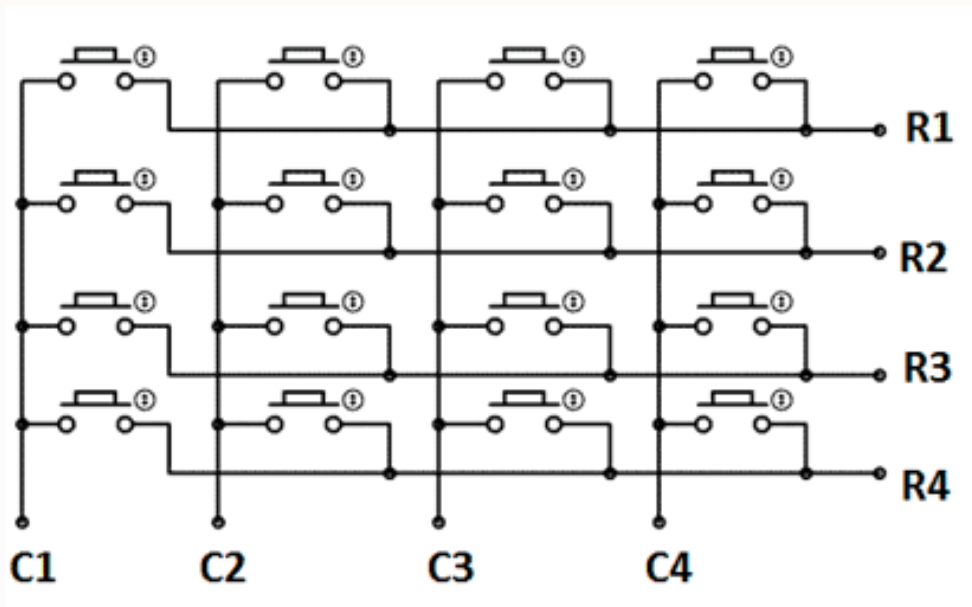
\includegraphics[width=0.5\textwidth]{4x4_button_layout.png}
    \caption*{4x4 Button Layout}
\end{figure}
\begin{figure}[H]
    \centering
    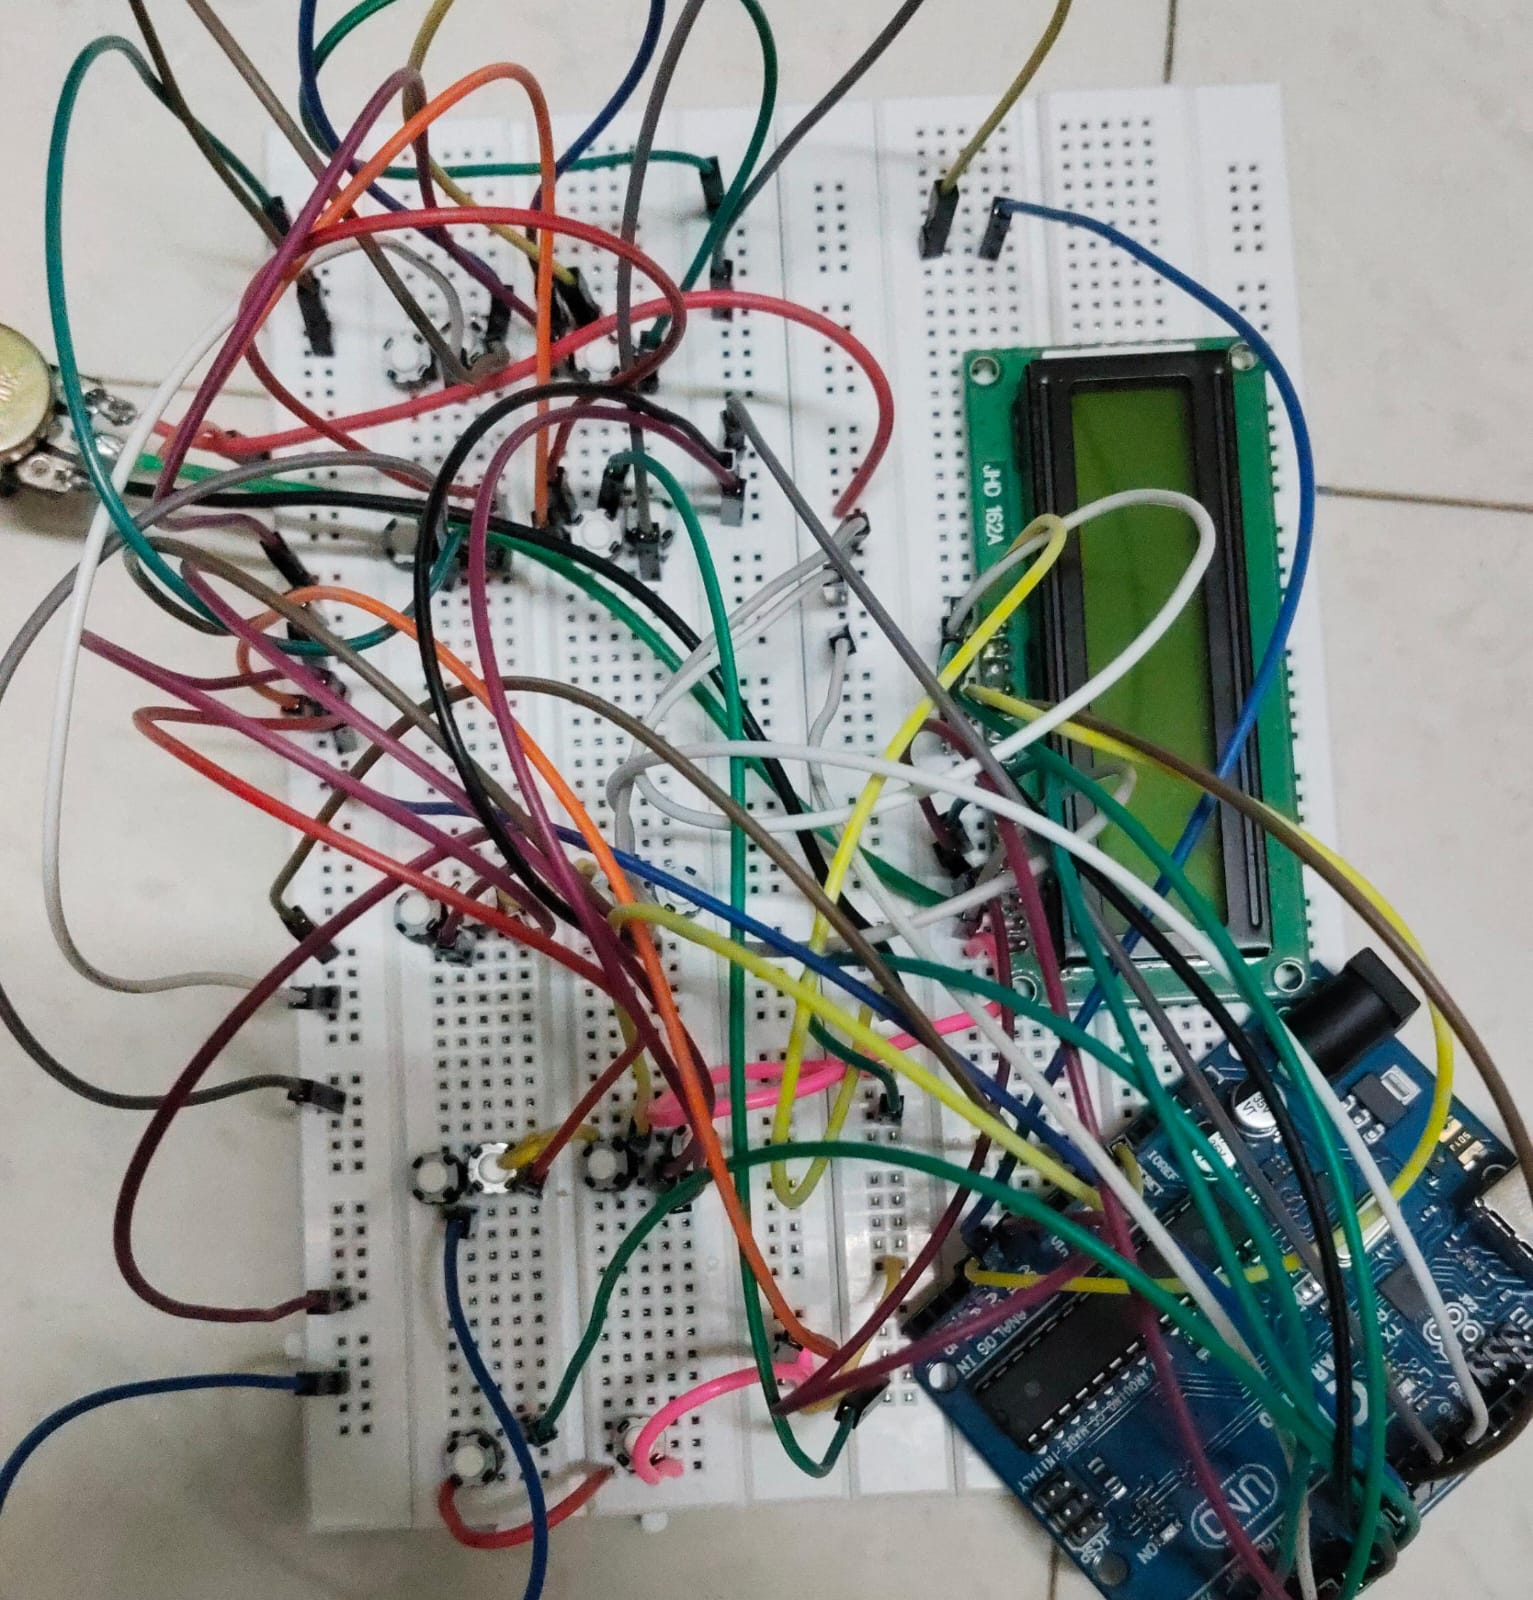
\includegraphics[width=0.4\textwidth]{sci_calc.jpeg}
    \caption*{Scientific Calculator Circuit}
\end{figure}
\section*{Reference}
The code has been referenced from https://github.com/EE24BTECH11012/EE1003/blob/\\c55818859eebe407cd8a028f4a39012ec59f1942/Hardware/Calculator/main.c
\end{document}
